%%%% Preamble %%%%
\documentclass[a4paper, oneside, 10pt]{article}

% wider text, smaller margins
\usepackage{a4wide}

% font choice
\usepackage[utf8]{inputenc}
% \usepackage{kpfonts}
\usepackage[T1]{fontenc}
% \usepackage{newtxtext,newtxmath}

% for coloring
\usepackage[dvipsnames]{xcolor}

% for index list
\usepackage{makeidx}
\makeindex

% for better lists
\usepackage{enumitem}

% for images
\usepackage{graphicx}
\graphicspath{{./Pics/}}

% for hyperrefs
\usepackage{hyperref}

% for declaring math operators
\usepackage{amsthm}

% wrap text around figures
\usepackage{wrapfig}

% chagne format of section titles
\usepackage{titlesec}

% algorithms
\usepackage[]{algorithm2e}

% \titleformat*{\section}{\LARGE\bfseries}
% \titleformat*{\subsection}{\Large\bfseries}
% \titleformat*{\subsubsection}{\large\bfseries}
\titleformat*{\paragraph}{\bfseries\itshape}
% \titleformat*{\subparagraph}{\large\bfseries}

% nice text boxes
\usepackage{tcolorbox}
\newtcbox{\note}{on line, boxrule=0pt, boxsep=0pt, arc=0pt, outer arc=0pt, left=1pt, right=1pt, top=2pt, bottom=2pt, fontupper=\itshape}
% \newtcolorbox{notebox}{boxrule=0pt}
\newtcolorbox{notebox}[1][colback=black!5]{boxrule=0pt, #1}

% biblatex seetings for better referencing
\usepackage[backend=biber,
            citestyle=authoryear,
            bibstyle=numeric,
            block=space,
            backref=true,
            date=year,
            maxcitenames=2,
            mincitenames=1,
            url=false,
            doi=false,
            isbn=false,
            eprint=false]{biblatex}
\addbibresource{refs.bib}


%%% theorem environments
\theoremstyle{plain}
\newtheoremstyle{mytheoremstyle} % name
    {\topsep}{\topsep}{}{}%
    {\bfseries}% Theorem head font
    {}{.5em}%
    {\thmname{#1}\thmnumber{ #2}\thmnote{ (#3)}}  % Theorem head spec (can be left empty, meaning ‘normal’)
\theoremstyle{mytheoremstyle}
\newtheorem{theorem}{Theorem}[section]

\theoremstyle{definition}
\newtheoremstyle{mydefstyle} % name
    {\topsep}{\partopsep}{}{}%
    {\bfseries}% Theorem head font
    {}{.5em}%
    {\thmname{#1}\thmnumber{ #2}\thmnote{ (#3)}}  % Theorem head spec (can be left empty, meaning ‘normal’)
\theoremstyle{mydefstyle}
\newtheorem{definition}{Definition}[section]

%%%%% NEW MATH DEFINITIONS %%%%%

\usepackage{amsmath,amsfonts,bm}

% Mark sections of captions for referring to divisions of figures
\newcommand{\figleft}{{\em (Left)}}
\newcommand{\figcenter}{{\em (Center)}}
\newcommand{\figright}{{\em (Right)}}
\newcommand{\figtop}{{\em (Top)}}
\newcommand{\figbottom}{{\em (Bottom)}}
\newcommand{\captiona}{{\em (a)}}
\newcommand{\captionb}{{\em (b)}}
\newcommand{\captionc}{{\em (c)}}
\newcommand{\captiond}{{\em (d)}}

% Highlight a newly defined term
\newcommand{\iterm}[1]{{\emph{#1}\index{#1}}}


% Figure reference, lower-case.
\def\figref#1{figure~\ref{#1}}
% Figure reference, capital. For start of sentence
\def\Figref#1{Figure~\ref{#1}}
\def\twofigref#1#2{figures \ref{#1} and \ref{#2}}
\def\quadfigref#1#2#3#4{figures \ref{#1}, \ref{#2}, \ref{#3} and \ref{#4}}
% Section reference, lower-case.
\def\secref#1{section~\ref{#1}}
% Section reference, capital.
\def\Secref#1{Section~\ref{#1}}
% Reference to two sections.
\def\twosecrefs#1#2{sections \ref{#1} and \ref{#2}}
% Reference to three sections.
\def\secrefs#1#2#3{sections \ref{#1}, \ref{#2} and \ref{#3}}
% % Reference to an equation, lower-case.
% \def\eqref#1{equation~\ref{#1}}
% % Reference to an equation, upper case
% \def\Eqref#1{Equation~\ref{#1}}
% % A raw reference to an equation---avoid using if possible
% \def\plaineqref#1{\ref{#1}}
% Reference to a chapter, lower-case.
\def\chapref#1{chapter~\ref{#1}}
% Reference to an equation, upper case.
\def\Chapref#1{Chapter~\ref{#1}}
% Reference to a range of chapters
\def\rangechapref#1#2{chapters\ref{#1}--\ref{#2}}
% Reference to an algorithm, lower-case.
\def\algref#1{algorithm~\ref{#1}}
% Reference to an algorithm, upper case.
\def\Algref#1{Algorithm~\ref{#1}}
\def\twoalgref#1#2{algorithms \ref{#1} and \ref{#2}}
\def\Twoalgref#1#2{Algorithms \ref{#1} and \ref{#2}}
% Reference to a part, lower case
\def\partref#1{part~\ref{#1}}
% Reference to a part, upper case
\def\Partref#1{Part~\ref{#1}}
\def\twopartref#1#2{parts \ref{#1} and \ref{#2}}

\def\ceil#1{\lceil #1 \rceil}
\def\floor#1{\lfloor #1 \rfloor}
\def\1{\bm{1}}
\newcommand{\train}{\mathcal{D}}
\newcommand{\valid}{\mathcal{D_{\mathrm{valid}}}}
\newcommand{\test}{\mathcal{D_{\mathrm{test}}}}

\def\eps{{\epsilon}}


% Random variables
\def\reta{{\textnormal{$\eta$}}}
\def\ra{{\textnormal{a}}}
\def\rb{{\textnormal{b}}}
\def\rc{{\textnormal{c}}}
\def\rd{{\textnormal{d}}}
\def\re{{\textnormal{e}}}
\def\rf{{\textnormal{f}}}
\def\rg{{\textnormal{g}}}
\def\rh{{\textnormal{h}}}
\def\ri{{\textnormal{i}}}
\def\rj{{\textnormal{j}}}
\def\rk{{\textnormal{k}}}
\def\rl{{\textnormal{l}}}
% rm is already a command, just don't name any random variables m
\def\rn{{\textnormal{n}}}
\def\ro{{\textnormal{o}}}
\def\rp{{\textnormal{p}}}
\def\rq{{\textnormal{q}}}
\def\rr{{\textnormal{r}}}
\def\rs{{\textnormal{s}}}
\def\rt{{\textnormal{t}}}
\def\ru{{\textnormal{u}}}
\def\rv{{\textnormal{v}}}
\def\rw{{\textnormal{w}}}
\def\rx{{\textnormal{x}}}
\def\ry{{\textnormal{y}}}
\def\rz{{\textnormal{z}}}

% Random vectors
\def\rvepsilon{{\mathbf{\epsilon}}}
\def\rvtheta{{\mathbf{\theta}}}
\def\rva{{\mathbf{a}}}
\def\rvb{{\mathbf{b}}}
\def\rvc{{\mathbf{c}}}
\def\rvd{{\mathbf{d}}}
\def\rve{{\mathbf{e}}}
\def\rvf{{\mathbf{f}}}
\def\rvg{{\mathbf{g}}}
\def\rvh{{\mathbf{h}}}
\def\rvu{{\mathbf{i}}}
\def\rvj{{\mathbf{j}}}
\def\rvk{{\mathbf{k}}}
\def\rvl{{\mathbf{l}}}
\def\rvm{{\mathbf{m}}}
\def\rvn{{\mathbf{n}}}
\def\rvo{{\mathbf{o}}}
\def\rvp{{\mathbf{p}}}
\def\rvq{{\mathbf{q}}}
\def\rvr{{\mathbf{r}}}
\def\rvs{{\mathbf{s}}}
\def\rvt{{\mathbf{t}}}
\def\rvu{{\mathbf{u}}}
\def\rvv{{\mathbf{v}}}
\def\rvw{{\mathbf{w}}}
\def\rvx{{\mathbf{x}}}
\def\rvy{{\mathbf{y}}}
\def\rvz{{\mathbf{z}}}

% Elements of random vectors
\def\erva{{\textnormal{a}}}
\def\ervb{{\textnormal{b}}}
\def\ervc{{\textnormal{c}}}
\def\ervd{{\textnormal{d}}}
\def\erve{{\textnormal{e}}}
\def\ervf{{\textnormal{f}}}
\def\ervg{{\textnormal{g}}}
\def\ervh{{\textnormal{h}}}
\def\ervi{{\textnormal{i}}}
\def\ervj{{\textnormal{j}}}
\def\ervk{{\textnormal{k}}}
\def\ervl{{\textnormal{l}}}
\def\ervm{{\textnormal{m}}}
\def\ervn{{\textnormal{n}}}
\def\ervo{{\textnormal{o}}}
\def\ervp{{\textnormal{p}}}
\def\ervq{{\textnormal{q}}}
\def\ervr{{\textnormal{r}}}
\def\ervs{{\textnormal{s}}}
\def\ervt{{\textnormal{t}}}
\def\ervu{{\textnormal{u}}}
\def\ervv{{\textnormal{v}}}
\def\ervw{{\textnormal{w}}}
\def\ervx{{\textnormal{x}}}
\def\ervy{{\textnormal{y}}}
\def\ervz{{\textnormal{z}}}

% Random matrices
\def\rmA{{\mathbf{A}}}
\def\rmB{{\mathbf{B}}}
\def\rmC{{\mathbf{C}}}
\def\rmD{{\mathbf{D}}}
\def\rmE{{\mathbf{E}}}
\def\rmF{{\mathbf{F}}}
\def\rmG{{\mathbf{G}}}
\def\rmH{{\mathbf{H}}}
\def\rmI{{\mathbf{I}}}
\def\rmJ{{\mathbf{J}}}
\def\rmK{{\mathbf{K}}}
\def\rmL{{\mathbf{L}}}
\def\rmM{{\mathbf{M}}}
\def\rmN{{\mathbf{N}}}
\def\rmO{{\mathbf{O}}}
\def\rmP{{\mathbf{P}}}
\def\rmQ{{\mathbf{Q}}}
\def\rmR{{\mathbf{R}}}
\def\rmS{{\mathbf{S}}}
\def\rmT{{\mathbf{T}}}
\def\rmU{{\mathbf{U}}}
\def\rmV{{\mathbf{V}}}
\def\rmW{{\mathbf{W}}}
\def\rmX{{\mathbf{X}}}
\def\rmY{{\mathbf{Y}}}
\def\rmZ{{\mathbf{Z}}}

% Elements of random matrices
\def\ermA{{\textnormal{A}}}
\def\ermB{{\textnormal{B}}}
\def\ermC{{\textnormal{C}}}
\def\ermD{{\textnormal{D}}}
\def\ermE{{\textnormal{E}}}
\def\ermF{{\textnormal{F}}}
\def\ermG{{\textnormal{G}}}
\def\ermH{{\textnormal{H}}}
\def\ermI{{\textnormal{I}}}
\def\ermJ{{\textnormal{J}}}
\def\ermK{{\textnormal{K}}}
\def\ermL{{\textnormal{L}}}
\def\ermM{{\textnormal{M}}}
\def\ermN{{\textnormal{N}}}
\def\ermO{{\textnormal{O}}}
\def\ermP{{\textnormal{P}}}
\def\ermQ{{\textnormal{Q}}}
\def\ermR{{\textnormal{R}}}
\def\ermS{{\textnormal{S}}}
\def\ermT{{\textnormal{T}}}
\def\ermU{{\textnormal{U}}}
\def\ermV{{\textnormal{V}}}
\def\ermW{{\textnormal{W}}}
\def\ermX{{\textnormal{X}}}
\def\ermY{{\textnormal{Y}}}
\def\ermZ{{\textnormal{Z}}}

% Vectors
\def\vzero{{\bm{0}}}
\def\vone{{\bm{1}}}
\def\vmu{{\bm{\mu}}}
\def\vtheta{{\bm{\theta}}}
\def\va{{\bm{a}}}
\def\vb{{\bm{b}}}
\def\vc{{\bm{c}}}
\def\vd{{\bm{d}}}
\def\ve{{\bm{e}}}
\def\vf{{\bm{f}}}
\def\vg{{\bm{g}}}
\def\vh{{\bm{h}}}
\def\vi{{\bm{i}}}
\def\vj{{\bm{j}}}
\def\vk{{\bm{k}}}
\def\vl{{\bm{l}}}
\def\vm{{\bm{m}}}
\def\vn{{\bm{n}}}
\def\vo{{\bm{o}}}
\def\vp{{\bm{p}}}
\def\vq{{\bm{q}}}
\def\vr{{\bm{r}}}
\def\vs{{\bm{s}}}
\def\vt{{\bm{t}}}
\def\vu{{\bm{u}}}
\def\vv{{\bm{v}}}
\def\vw{{\bm{w}}}
\def\vx{{\bm{x}}}
\def\vy{{\bm{y}}}
\def\vz{{\bm{z}}}

% Elements of vectors
\def\evalpha{{\alpha}}
\def\evbeta{{\beta}}
\def\evepsilon{{\epsilon}}
\def\evlambda{{\lambda}}
\def\evomega{{\omega}}
\def\evmu{{\mu}}
\def\evpsi{{\psi}}
\def\evsigma{{\sigma}}
\def\evtheta{{\theta}}
\def\eva{{a}}
\def\evb{{b}}
\def\evc{{c}}
\def\evd{{d}}
\def\eve{{e}}
\def\evf{{f}}
\def\evg{{g}}
\def\evh{{h}}
\def\evi{{i}}
\def\evj{{j}}
\def\evk{{k}}
\def\evl{{l}}
\def\evm{{m}}
\def\evn{{n}}
\def\evo{{o}}
\def\evp{{p}}
\def\evq{{q}}
\def\evr{{r}}
\def\evs{{s}}
\def\evt{{t}}
\def\evu{{u}}
\def\evv{{v}}
\def\evw{{w}}
\def\evx{{x}}
\def\evy{{y}}
\def\evz{{z}}

% Matrix
\def\mA{{\bm{A}}}
\def\mB{{\bm{B}}}
\def\mC{{\bm{C}}}
\def\mD{{\bm{D}}}
\def\mE{{\bm{E}}}
\def\mF{{\bm{F}}}
\def\mG{{\bm{G}}}
\def\mH{{\bm{H}}}
\def\mI{{\bm{I}}}
\def\mJ{{\bm{J}}}
\def\mK{{\bm{K}}}
\def\mL{{\bm{L}}}
\def\mM{{\bm{M}}}
\def\mN{{\bm{N}}}
\def\mO{{\bm{O}}}
\def\mP{{\bm{P}}}
\def\mQ{{\bm{Q}}}
\def\mR{{\bm{R}}}
\def\mS{{\bm{S}}}
\def\mT{{\bm{T}}}
\def\mU{{\bm{U}}}
\def\mV{{\bm{V}}}
\def\mW{{\bm{W}}}
\def\mX{{\bm{X}}}
\def\mY{{\bm{Y}}}
\def\mZ{{\bm{Z}}}
\def\mBeta{{\bm{\beta}}}
\def\mPhi{{\bm{\Phi}}}
\def\mLambda{{\bm{\Lambda}}}
\def\mSigma{{\bm{\Sigma}}}

% Tensor
\DeclareMathAlphabet{\mathsfit}{\encodingdefault}{\sfdefault}{m}{sl}
\SetMathAlphabet{\mathsfit}{bold}{\encodingdefault}{\sfdefault}{bx}{n}
\newcommand{\tens}[1]{\bm{\mathsfit{#1}}}
\def\tA{{\tens{A}}}
\def\tB{{\tens{B}}}
\def\tC{{\tens{C}}}
\def\tD{{\tens{D}}}
\def\tE{{\tens{E}}}
\def\tF{{\tens{F}}}
\def\tG{{\tens{G}}}
\def\tH{{\tens{H}}}
\def\tI{{\tens{I}}}
\def\tJ{{\tens{J}}}
\def\tK{{\tens{K}}}
\def\tL{{\tens{L}}}
\def\tM{{\tens{M}}}
\def\tN{{\tens{N}}}
\def\tO{{\tens{O}}}
\def\tP{{\tens{P}}}
\def\tQ{{\tens{Q}}}
\def\tR{{\tens{R}}}
\def\tS{{\tens{S}}}
\def\tT{{\tens{T}}}
\def\tU{{\tens{U}}}
\def\tV{{\tens{V}}}
\def\tW{{\tens{W}}}
\def\tX{{\tens{X}}}
\def\tY{{\tens{Y}}}
\def\tZ{{\tens{Z}}}


% Graph
\def\gA{{\mathcal{A}}}
\def\gB{{\mathcal{B}}}
\def\gC{{\mathcal{C}}}
\def\gD{{\mathcal{D}}}
\def\gE{{\mathcal{E}}}
\def\gF{{\mathcal{F}}}
\def\gG{{\mathcal{G}}}
\def\gH{{\mathcal{H}}}
\def\gI{{\mathcal{I}}}
\def\gJ{{\mathcal{J}}}
\def\gK{{\mathcal{K}}}
\def\gL{{\mathcal{L}}}
\def\gM{{\mathcal{M}}}
\def\gN{{\mathcal{N}}}
\def\gO{{\mathcal{O}}}
\def\gP{{\mathcal{P}}}
\def\gQ{{\mathcal{Q}}}
\def\gR{{\mathcal{R}}}
\def\gS{{\mathcal{S}}}
\def\gT{{\mathcal{T}}}
\def\gU{{\mathcal{U}}}
\def\gV{{\mathcal{V}}}
\def\gW{{\mathcal{W}}}
\def\gX{{\mathcal{X}}}
\def\gY{{\mathcal{Y}}}
\def\gZ{{\mathcal{Z}}}

% Sets
\def\sA{{\mathbb{A}}}
\def\sB{{\mathbb{B}}}
\def\sC{{\mathbb{C}}}
\def\sD{{\mathbb{D}}}
% Don't use a set called E, because this would be the same as our symbol
% for expectation.
\def\sF{{\mathbb{F}}}
\def\sG{{\mathbb{G}}}
\def\sH{{\mathbb{H}}}
\def\sI{{\mathbb{I}}}
\def\sJ{{\mathbb{J}}}
\def\sK{{\mathbb{K}}}
\def\sL{{\mathbb{L}}}
\def\sM{{\mathbb{M}}}
\def\sN{{\mathbb{N}}}
\def\sO{{\mathbb{O}}}
\def\sP{{\mathbb{P}}}
\def\sQ{{\mathbb{Q}}}
\def\sR{{\mathbb{R}}}
\def\sS{{\mathbb{S}}}
\def\sT{{\mathbb{T}}}
\def\sU{{\mathbb{U}}}
\def\sV{{\mathbb{V}}}
\def\sW{{\mathbb{W}}}
\def\sX{{\mathbb{X}}}
\def\sY{{\mathbb{Y}}}
\def\sZ{{\mathbb{Z}}}

% Entries of a matrix
\def\emLambda{{\Lambda}}
\def\emA{{A}}
\def\emB{{B}}
\def\emC{{C}}
\def\emD{{D}}
\def\emE{{E}}
\def\emF{{F}}
\def\emG{{G}}
\def\emH{{H}}
\def\emI{{I}}
\def\emJ{{J}}
\def\emK{{K}}
\def\emL{{L}}
\def\emM{{M}}
\def\emN{{N}}
\def\emO{{O}}
\def\emP{{P}}
\def\emQ{{Q}}
\def\emR{{R}}
\def\emS{{S}}
\def\emT{{T}}
\def\emU{{U}}
\def\emV{{V}}
\def\emW{{W}}
\def\emX{{X}}
\def\emY{{Y}}
\def\emZ{{Z}}
\def\emSigma{{\Sigma}}

% entries of a tensor
% Same font as tensor, without \bm wrapper
\newcommand{\etens}[1]{\mathsfit{#1}}
\def\etLambda{{\etens{\Lambda}}}
\def\etA{{\etens{A}}}
\def\etB{{\etens{B}}}
\def\etC{{\etens{C}}}
\def\etD{{\etens{D}}}
\def\etE{{\etens{E}}}
\def\etF{{\etens{F}}}
\def\etG{{\etens{G}}}
\def\etH{{\etens{H}}}
\def\etI{{\etens{I}}}
\def\etJ{{\etens{J}}}
\def\etK{{\etens{K}}}
\def\etL{{\etens{L}}}
\def\etM{{\etens{M}}}
\def\etN{{\etens{N}}}
\def\etO{{\etens{O}}}
\def\etP{{\etens{P}}}
\def\etQ{{\etens{Q}}}
\def\etR{{\etens{R}}}
\def\etS{{\etens{S}}}
\def\etT{{\etens{T}}}
\def\etU{{\etens{U}}}
\def\etV{{\etens{V}}}
\def\etW{{\etens{W}}}
\def\etX{{\etens{X}}}
\def\etY{{\etens{Y}}}
\def\etZ{{\etens{Z}}}

% The true underlying data generating distribution
\newcommand{\pdata}{p_{\rm{data}}}
% The empirical distribution defined by the training set
\newcommand{\ptrain}{\hat{p}_{\rm{data}}}
\newcommand{\Ptrain}{\hat{P}_{\rm{data}}}
% The model distribution
\newcommand{\pmodel}{p_{\rm{model}}}
\newcommand{\Pmodel}{P_{\rm{model}}}
\newcommand{\ptildemodel}{\tilde{p}_{\rm{model}}}
% Stochastic autoencoder distributions
\newcommand{\pencode}{p_{\rm{encoder}}}
\newcommand{\pdecode}{p_{\rm{decoder}}}
\newcommand{\precons}{p_{\rm{reconstruct}}}

\newcommand{\laplace}{\mathrm{Laplace}} % Laplace distribution

\newcommand{\E}{\mathbb{E}}
\newcommand{\Ls}{\mathcal{L}}
\newcommand{\R}{\mathbb{R}}
\newcommand{\emp}{\tilde{p}}
\newcommand{\lr}{\alpha}
\newcommand{\reg}{\lambda}
\newcommand{\rect}{\mathrm{rectifier}}
\newcommand{\softmax}{\mathrm{softmax}}
\newcommand{\sigmoid}{\sigma}
\newcommand{\softplus}{\zeta}
\newcommand{\KL}{D_{\mathrm{KL}}}
\newcommand{\Var}{\mathrm{Var}}
\newcommand{\standarderror}{\mathrm{SE}}
\newcommand{\Cov}{\mathrm{Cov}}
\newcommand{\logb}{\log_2}
% Wolfram Mathworld says $L^2$ is for function spaces and $\ell^2$ is for vectors
% But then they seem to use $L^2$ for vectors throughout the site, and so does
% wikipedia.
\newcommand{\normlzero}{L^0}
\newcommand{\normlone}{L^1}
\newcommand{\normltwo}{L^2}
\newcommand{\normlp}{L^p}
\newcommand{\normmax}{L^\infty}

\newcommand{\parents}{Pa} % See usage in notation.tex. Chosen to match Daphne's book.

\DeclareMathOperator*{\argmax}{arg\,max}
\DeclareMathOperator*{\argmin}{arg\,min}

\DeclareMathOperator{\sign}{sign}
\DeclareMathOperator{\Tr}{Tr}
\let\ab\allowbreak

%%% new shorthand commands
\newcommand{\nn}{\nonumber \\}%

\newcommand{\tldr}{\textbf{TLDR: }}
\newcommand{\concl}{\textbf{Concluding remarks: }}


\begin{document}

% where pics are
\graphicspath{ {./Pics/} }

% supress paragraph idents
\setlength{\parindent}{0pt}
\setlength{\parskip}{1ex plus 0.5ex minus 0.2ex}

% Number equations within a section
\numberwithin{equation}{section}

{\large Magda's notes about papers read in \textbf{2022}}

{\hfill Last update: \today}

Informal notes for my future self who is likely to forget.
I explain the papers the way I understand them, using terminology and logic natural to me.
This means I may deviate from the original paper structure, notation, etc.
At places, my interpretation my be incorrect due to lack of understanding. 
I will strive for this not to happen too often but I'm certainly not infallible. 

This is a working document, not  polished, with possible typos, editing errors, etc.

Imagery is usually taken directly from the original papers (unless otherwise stated).


% Print table of contents
\tableofcontents

\clearpage

\section{graphNVP}\label{sec:graphNVP}\index{graphNVP}

\begin{notebox}
\textbf{Paper: } \fullcite{madhawa_graphnvp_2019}
\vspace{5pt}

\href{https://openreview.net/forum?id=ryxQ6T4YwB}{ICLR not accept reviews}
\hspace{1cm}
\href{https://github.com/pfnet-research/graph-nvp}{Official code}
\hspace{1cm}
\href{run:/home/magda/Dropbox/Zot/Madhawa et al_2019_GraphNVP.pdf}{Local pdf}

\hfill Notes taken: 6/2/2022 \index{February 2022}
\end{notebox}

\begin{notebox}[colback=red!5]
\tldr Generate graphs\index{graph} $G = (A, X)$ through invertible flows\index{invertible flow}. Dequantize\index{dequantize} A and X by uniform noise to make modelling continuous. Coupling strategy splitting the A and X matrices always by one node vs all the rest (breaks permutation invariance). The scale and translation in the coupling are graph NNs (do not have to be invertible) - for X functions of all other nodes and complete A matrix; for A edges between other nodes. Final reconstructed / generated A, X are quantized (floored) to get back to discrete.
\end{notebox}

\begin{notebox}[colback=yellow!5]
\textbf{Notes:} 
\begin{itemize}[nosep]
\item Dequantize by simple uniform noise to get rid of the discreteness problem, then simply quantize (floor) to get back.
\item ZINC-250K random sample of 250k molecules from complete ZINC to make experiments manageable. 
\item Good list of baseline models for experiments
\item No validation checks during generation $\to$ versatile and fast.
\item Coupling structure by nodes breaks permutation invariance - is this really a problem?
\end{itemize}
\end{notebox}

\begin{figure}[ht]
\centering
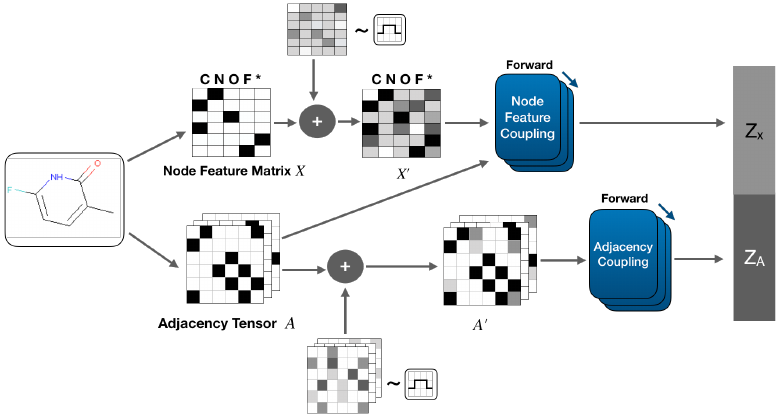
\includegraphics[width=10cm]{graphNVP_Figure1.png}
\caption{For the forward transform, A and X matrices are perturbed by uniform noise. The node coupling is conditioned on the A matrix.}
\end{figure}

\begin{figure}[ht]
\centering
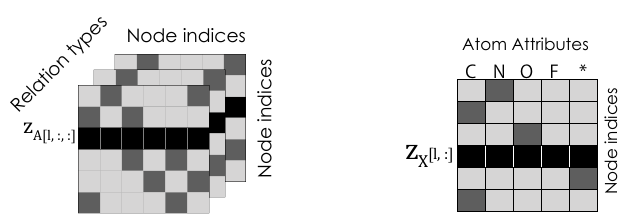
\includegraphics[width=6cm]{graphNVP_Figure2.png}
\caption{The coupling structure splits the A and X matrices as one node vs all the rest. This works best in experiments, though breaks down permutation invariance.}
\end{figure}

\begin{figure}[ht]
\centering
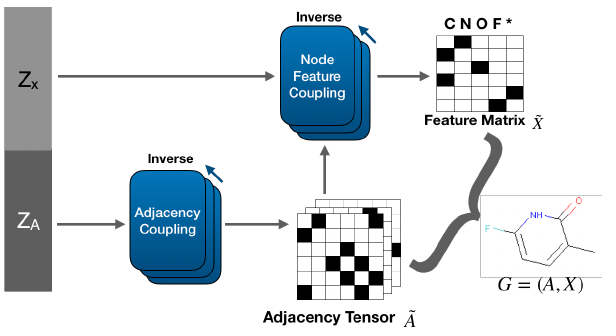
\includegraphics[width=8cm]{graphNVP_Figure3.png}
\caption{Generation is in two steps because the reverse coupling transform of X is conditioned on A so this needs to be generated first. Using simple dequantization (flooring) to get from continuous flow output to discrete A, X.}
\end{figure}

\textbf{Experiments:} on QM9\index{QM9} and ZINC-250K\index{ZINC} with kekulized graphs (without hydrogens) - our \emph{cheat} version.
Have not so great validity but high uniqueness.
Claim benefits in speed of generation as opposed models that have complex decoders checking the validity of molecules in the process.
Some comments on smoothness of latent space and possibility to interpolate for property control but not very convincing.


\clearpage

\section{MPGVAE}\label{sec:MPGVAE}\index{MPGVAE}

\begin{notebox}
\textbf{Paper: } \fullcite{flam-shepherd_mpgvae_2021}
\vspace{5pt}

no reviews
\hspace{1cm}
no official code
\hspace{1cm}
\href{Flam-Shepherd et al_2021_MPGVAE.pdf}{Local pdf}

\hfill Notes taken: 6/2/2022 \index{February 2022}
\end{notebox}

\begin{notebox}[colback=red!5]
\tldr Builts on GraphVAE (Simonovsky and Komodakis, 2018) but bypasses the graph matching problem by relaying on message passing NN in encoder and decoder so that the reconstruction loss can be calculated directly. Message passing over edges, nodes use attention to aggregate these.
To get from node representation to laten vector they use set2vec\index{set2vec} from Vinyals 2015 to be invariant to the node ordering.
To get from latent back to graph they use simply linear layer and then message passing, finishing with softmax over node and egde representation to create stochastic edge and node graph representations from which the graphs can be samples (in practice assume by max category).
The reconstruction loss assumes independence of node and edge features $p\theta(G|z) = \Pi_{v \in G} p(x_v | z) \Pi_{u \in G} p(e_{uv} | z)$
\end{notebox}

\begin{notebox}[colback=yellow!5]
\textbf{Notes:} 
\begin{itemize}[nosep]
\item code not publicly available - asked first author, no answer
\item set2vec to be invariant to node ordering when getting from the node representation in the last MPNN layer the latent representation $z$, on the way back can use use MLP and MPNN cause the ordering problem was solved when moving to the latent
\item \emph{\textbf{I still do not see how the reconstruction loss can be evaluated. Even with the independence assumptions, each of the node/ edge likelihoods has to be matched to the respective edge/ node in the original graph. How can this be done without some matching procedure?}}
\end{itemize}
\end{notebox}


Graph with adjacency matrix, edge feature tensor and node feature matrix $G = (A, E, X)$.
Assume independence between node and edge probability distributions (Erdos-R\'enyi graph model) such as in \citetitle{simonovsky_graphvae_2018} of \textcite{simonovsky_graphvae_2018}\index{GraphVAE}.

Starting point is standard VAE and ELBO. Both edge and node features are categorical.
Build a message passing NN (MPNN)\index{message passing NN} into encoder and decoder of the VAE.

Refers to Graphite from Grover et al 2018 as nearest baseline - how different is this?

\begin{figure}[ht]
\centering
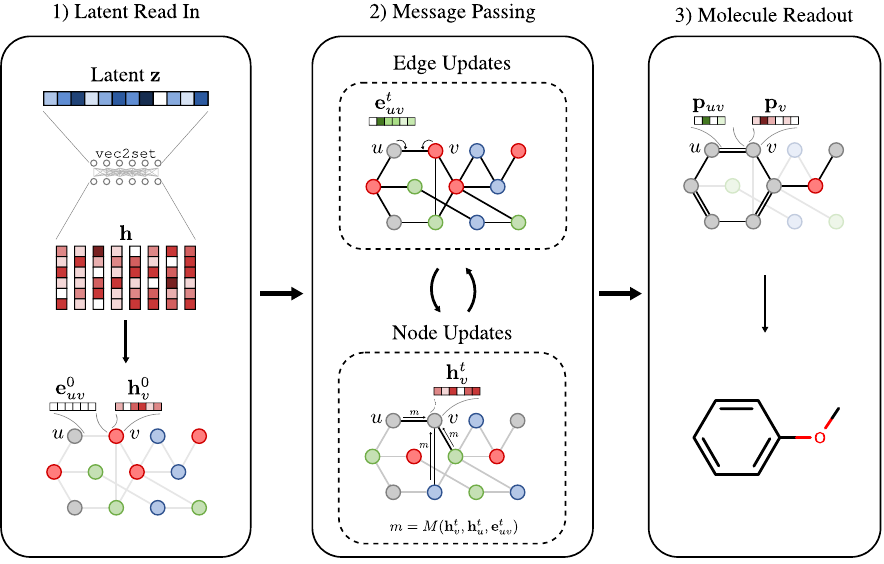
\includegraphics[width=10cm]{mpgvae_figure1.png}
\caption{1) Read in latent $z$ by passing it through linear layer to get to correct node dimensions and pass it through RNN to get initial node featues. Edge features fixed to zero - unconnected graph. 2) Message passing on both, node and edge representations. 3) Use last node and edge representation to predict independent node and edge feature probabilities.}
\end{figure}

Claim that has lower complexity than GrpahVAE (how so?).

\textbf{Encoder:} Use MPNN to map node and edge representations into latent space.
Messages are constructed at edge level as linear functions of itself, neighbouring nodes, and edge features passed through tanh nonlinearity.
Edge updates are directly the messages. 
Node updates first use attention to reweight the messages and then pass it through a GRUCell (this is not very clear, there is something strange in eq. 11 - should be a message for u only? not uv?)
Use set2set from Vinyals 2015 (unlike in seq2seq, in sets the order should not matter and the model should produce the same representation in arbitrary ordering of the set) to read from last node representation to fixed-sized hidden representation $z$.

\textbf{Decoder:} Pass latent through linear layer to expand dims and then RNN to get initial node featurs (edge features zero - unconnected graph). MPNN identical to encoder - update both nodes and eges.
Readout the last layer into stochastic graph representation by passing it through single layer NN and softmax.

\textbf{Experiments:} Over QM9 (not clear whether kekulized or not and if has hydrogens) - best validity compared to GrphVAE, MolGAN, CharacterVAE and Grammar VAE. Generate $10^4$ molecules and achieve validity over 90\%, unique almost 70\% and novel about 50\% - much better then baseline. 
Also evaluates the continuous (chemical properties) and discrete (avg number of atom types and ring size) property distributions of generated vs training sample graphs - claim to have both better than baseline.






\clearpage 
\printbibliography



% print index
\phantomsection
\cleardoublepage
\addcontentsline{toc}{section}{\indexname}
\printindex

\end{document}
